\documentclass[a1paper]{tikzposter}

\usetheme{Steph}

% Packages
\usepackage[T1]{fontenc}
\usepackage[utf8]{inputenc}
\usepackage{natbib,mdframed,amsmath,calc,graphicx,amssymb,relsize,multirow,rotating,bm,url,multicol,array,subfigure,eurosym}
\usepackage{tikz}
\usetikzlibrary{arrows,patterns, calc, arrows.meta}
\tikzset{>={Latex[width=3mm,length=5mm]}}

\renewcommand{\rmdefault}{phv}
\renewcommand{\sfdefault}{phv} 
\renewcommand{\labelitemi}{$\bullet$}

\newcommand{\compresslist}{
    \setlength{\itemsep}{1pt}
	\setlength{\parskip}{0pt}
	\setlength{\parsep}{0pt}
}

\definecolor{IGNVert}{RGB}{163, 210,  11}
\definecolor{IGNGris}{RGB}{159, 164, 168}
\definecolor{IGNGrisFonce}{RGB}{101, 105, 110}



\title{Conceptualising a co-operative building evolution dashboard on city regions over the past decades for densification studies}
\author{Bénédicte Bucher$^{1}$, Mouhamadou Ndim$^{1}$, Ana-Maria Olteanu-Raimond$^{1}$, Juste Raimbault$^{1, \ast}$, Julien Perret$^{1}$, Sebastian Dembski$^{2}$, Mathias Jehling$^{3}$}
\institute{$^{1}$ LASTIG, Univ. Gustave Eiffel, IGN-ENSG\\
$^{2}$ University of Liverpool\\
$^{3}$ Leibniz Institute of Ecological Urban and Regional Development\\\vspace*{0.5em}
$^{\ast}$ \texttt{juste.raimbault@ign.fr}
}
\titlegraphic{}

% Layout of title and logos, some other possible logos are available in images folder
% Don't hesitate to modify the positions if it doesn't suit you
\makeatletter
\renewcommand\TP@maketitle{
    \vspace*{-7cm}
    
    \hspace{.2\textwidth}
    
	\begin{tabular}{lcl}
	    %logo box 1
    	\begin{minipage}[b][.15\textheight][b]{.1\textwidth}

            
        	
\includegraphics[width=\linewidth]{./figures/LOGO_IGN}\\
            
             \vspace{1cm}
            
            
\includegraphics[width=\linewidth]{./figures/lastig}

            
    	\end{minipage}
    	&
    	%title box
    	\begin{minipage}[b][.2\textheight][b]{.75\textwidth}
    		\centering
    		\color{titlefgcolor}
      
            
    		{\bfseries \LARGE \sc Conceptualising a co-operative building evolution\par}
    		
    		{\bfseries \LARGE \sc dashboard on city regions over the past decades for densification studies \par}
    		\vspace*{1em}
    		{\Large \@author \par}
    		\vspace*{0.5em}
    		{\large \@institute}
    		
    	\end{minipage}
    	&
    	%logo box 2
    	\begin{minipage}[b][.15\textheight][b]{.1\textwidth}

                \vfill
     
            	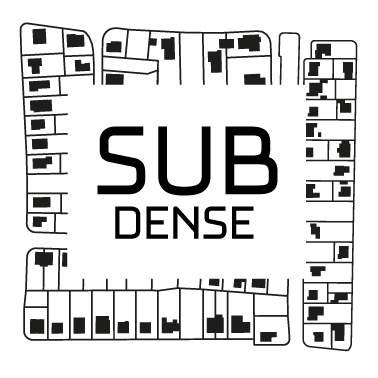
\includegraphics[width=1\textwidth]{./figures/subdense_Logo}

                \vfill
                \vfill
             
    	\end{minipage}
	\end{tabular}
}
\makeatother

%%%%%%%%%%%%%%%%%%%%%%%%%%%%%%%%%%%%%%%%%%%%%%%%%%%%%%%%%%%%%%%%%%%%%%%%%%%%%%%%
% Multicol Settings
%%%%%%%%%%%%%%%%%%%%%%%%%%%%%%%%%%%%%%%%%%%%%%%%%%%%%%%%%%%%%%%%%%%%%%%%%%%%%%%%
\setlength{\columnsep}{1.5em}
\setlength{\columnseprule}{0mm}

%%%%%%%%%%%%%%%%%%%%%%%%%%%%%%%%%%%%%%%%%%%%%%%%%%%%%%%%%%%%%%%%%%%%%%%%%%%%%%%%
% Save space in lists. Use this after the opening of the list
%%%%%%%%%%%%%%%%%%%%%%%%%%%%%%%%%%%%%%%%%%%%%%%%%%%%%%%%%%%%%%%%%%%%%%%%%%%%%%%%


% To remove the "latex tikz poster" at the bottom right corner
\tikzposterlatexaffectionproofoff

\begin{document}
	% Title block with title, author, logo, etc.
	\maketitle
	
%------------------------------------------------------
%----------------LINE 1--------------------------------
%------------------------------------------------------
% block alone on its line so you don't have to specify the columns environment

\vspace*{-5cm}

		%==============================================
		\block[titlewidthscale=0.5]{Context: The SubDense project}{

            
			\begin{itemize}
				\item Suburban densification can yield more \emph{sustainable cities} while avoiding issues linked to over-densification in centres.
				\item \emph{Multiple rationalities} of involved stakeholders (landowners, policy-makers) imply considerable \emph{planning challenges}.
			\end{itemize}

                 \bigskip

                The \textbf{SubDense} European project aims at better understanding how diverse \textbf{strategies of land policy} shape suburban densification across different \textbf{planning systems} (France, Germany, UK), from qualitative and quantitative viewpoints, looking in particular at \textbf{urban change dynamics at the building level} in 6 comparable city regions in these countries.

                \bigskip

                % However, the use of building data products require an expert knowledge for a proper application to change detection, including specification details and changes in these specifications. Furthermore, experts from different countries must be able to share this knowledge and their interpretation. They also should be able to share and reproduce quantitative analysis. Finally, concepts with multiple definitions, such as suburbia or densification itself, should be discussed between experts to reach a consensus on what is studied.

                \textbf{Research question:} \textit{how to ensure in that context the sharing of expert knowledge on different data specifications across countries, of diverse interpretations, analysis methods and tools, and of concepts with multiple definitions?}
   
		}
		%==============================================

  

	
	%==============================================
	\block[titlewidthscale=0.5]{Collaborative dashboard}{
		\parbox{0.33\textwidth}{
			\begin{mdframed}
                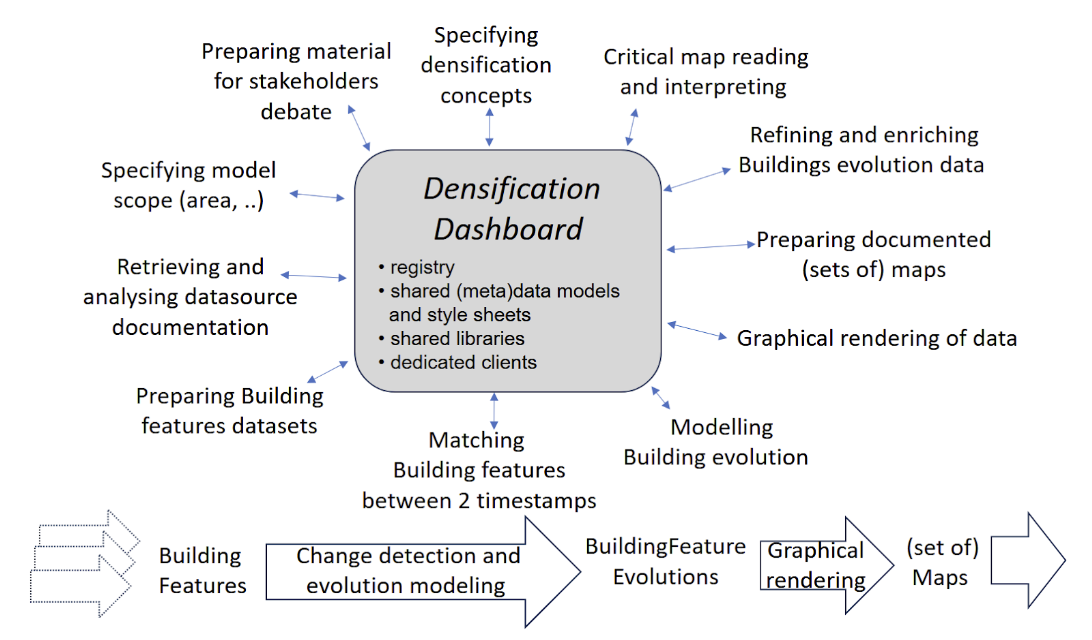
\includegraphics[width=\linewidth]{figures/dashboard.png}
		      \end{mdframed}
            }
         \hspace{0.5cm}
		\parbox{0.54\textwidth}{
            
            $\rightarrow$ A \textbf{collaborative dashboard} as a medium to \textbf{facilitate collaboration} between partners, \textbf{share methods, data and metadata}, and ensure reproducibility.

            \bigskip

            % The scope and functionalities of the dashboard are defined through an iterative a co-operative process, by considering ``User Stories'' that detail the expected contributions and motivation of different dashboard contributors and users. For example, qualitative researchers in urban policy act more as map readers and need to communicate their interpretations with local stakeholders, while a quantitative urban analyst will seek to run algorithms for change detection on multiple data sources, to finally produce maps used by the former. We show in Fig.~\ref{fig:dashboard} the current state of dashboard functionalities and usage, which can always evolve in the future.

            $\rightarrow$ Scope and functionalities of the dashboard defined iteratively by constructing ``User Stories'' with dashboard contributors and users.

            \bigskip
             
            % The core components of the dashboard are: (i) a registry for concepts, maps,  datasources, datasets, processes ; (ii) shared models for describing these items  ; (iii) shared libraries and software for computing building evolution and producing maps ; (iv) different clients to interact with the previous components (including a web application displaying maps, which corresponds to the more classical view of a ``dashboard'').

            $\rightarrow$ Core components are \textbf{registries} for concepts, maps, datasources, datasets, processes; shared \textbf{models} describing these; shared \textbf{libraries and software}; diverse \textbf{clients} to interact with these.
   
		}
		%==============================================
	}


        \block[titlewidthscale=0.5]{Architecture and implementation}{
            \parbox{0.3\textwidth}{
			\begin{mdframed}
                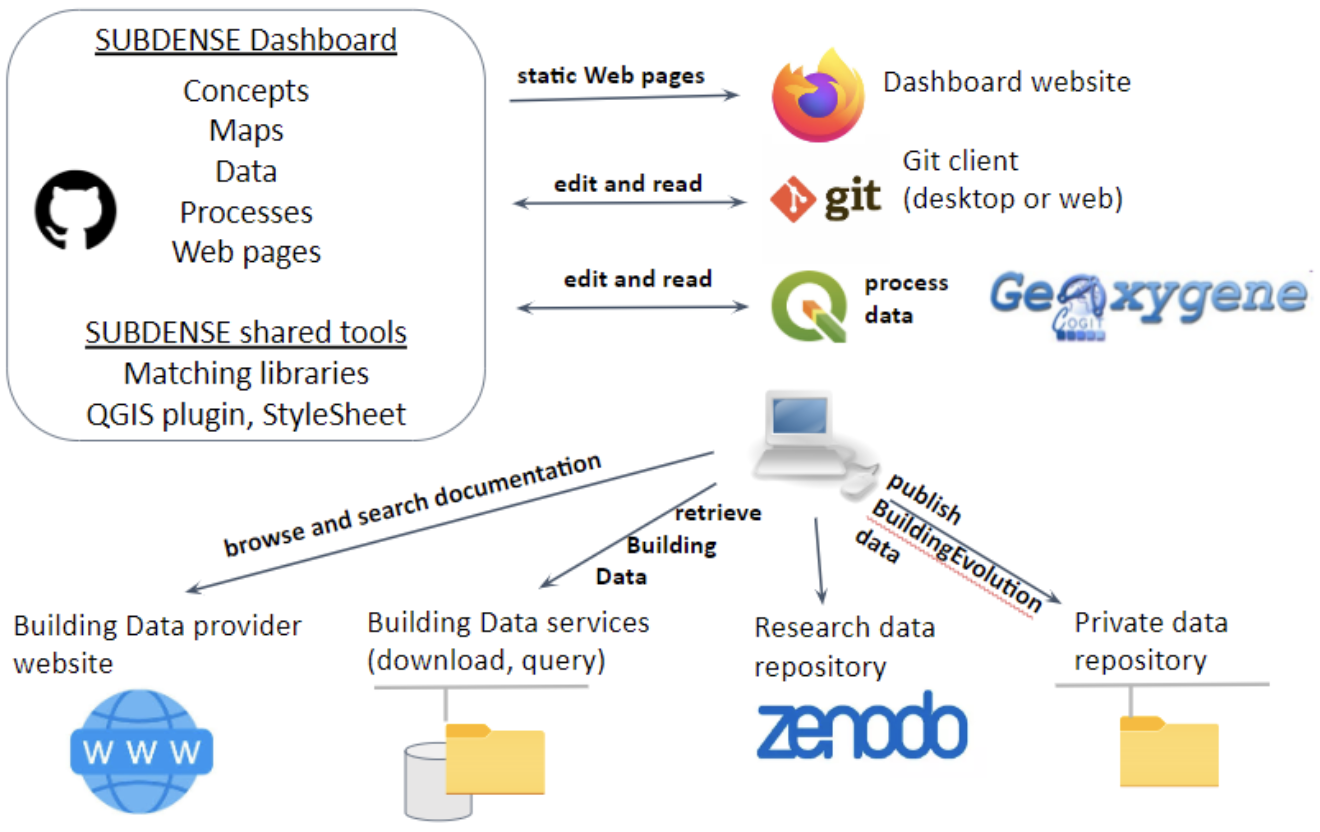
\includegraphics[width=\linewidth]{figures/archi.png}
		      \end{mdframed}
            }
            \hspace{0.5cm}
		\parbox{0.6\textwidth}{
         
			$\rightarrow$ The \textbf{git-based architecture} for the dashboard ensures tractability, reproducibility, and collaboration: core registries are stored and edited in a shared git repository: \url{https://github.com/subdense}.

            \bigskip

            % At this stage, three types of clients are proposed to interact with the dashboard: (i) the git client itself, by directly committing changes to the repository; (ii) a website, deployed automatically through github pages at \url{https://subdense.github.io/dashboard/}, for which user feedback is collected using a Javascript git library (currently under implementation); (iii) the open software QGIS for processing data, map reading and enrichment (python plugins for QGIS which run processes from the dashboard are also currently being implemented, and map style sheets are provided).
    
            $\rightarrow$ Clients implement interactions with the core and functionalities needed by partners for data analysis and integration (running change detection algorithms, adding data, exploring results and maps, providing Geospatial User Feedback, \ldots): \textbf{git clients} for direct edition; a \textbf{website} at \url{https://subdense.github.io/dashboard/} to explore results and provide feedback; \textbf{QGIS plugins} to run algorithms.


           % $\rightarrow$ An iterative process to produce \textbf{user stories}, finally leading to some specifications for the core architecture and functionalities of clients.

            }

        }

         

		%==============================================
		\block[titlewidthscale=0.95]{Application: Building change detection and Geospatial User Feedback}{

                %Processes in the dashboard include step-by-step descriptions of how a user retrieved data, processed it, produce maps, etc., but furthermore automated processes to run algorithms analysing data. One key process is change detection in building data, for which we use vector data matching algorithms \citep{olteanu2015knowledge}. Building features between two dates are matched using the Geometric Matching of Areas algorithm \citep{harvey1998geometric}, are then automatically interpreted as changes following a \texttt{BuildingFeatureEvolution} model following \cite{claramunt1997qualitative}, and finally filtered to distinguish specific cases of evolutions due to changes in data sources (for example, for France IGN BDTOPO changed between 2011 and 2021 the minimum threshold to include buildings and the way to compute building boundaries).


                %Maps are then produced using QGIS, and experts can provide Geospatial User Feedback (GUF) \citep{zabala2021geospatial}, either to rework the data model, to refine the automatic interpretation process, or more generally to gain knowledge on data quality or the process itself. Such an example of GUF is shown in fig.~\ref{fig:guf}, with the example of a specific area in Liverpool for which a local spatial planning expert went on the field and checked planning documents, to invalidate a building evolution produced by the algorithm. This feedback will then be used to reconsider the algorithm parametrisation or its internal mechanisms.

            \begin{itemize}
                \item \textbf{Geospatial data matching} algorithms (Geoxygene library) for \textbf{building change detection} between 2011 and 2021.
                \item \textbf{Geospatial User Feedback} collected from experts on produced evolution maps, to \textbf{improve} data analysis workflows.
            \end{itemize}
  
			
		}
		
	
		
	
	
\node [above right,outer sep=20pt,minimum width=\textwidth,align=center,draw=none,fill=none, text = IGNGrisFonce] at (bottomleft) {\centering \huge \bf AGILE 2024};

\end{document}

\endinput


% Future work 

\begin{itemize}
				\item \emph{heterogeneous data integration} \cite{bucher2021towards}, to couple densification analysis with socio-economic data;
                \item develop and explore \emph{simulation models} for the impact of policies on densification processes, parametrise these models with the qualitative data obtained through interviews during the project.
			\end{itemize}



	%==============================================
		% bibliography managed with natbib
		\block[titlewidthscale=0.3,bodyoffsety=1.8cm,titleoffsety=.1cm]{References}{
			% This command is to prevent the printing of a second "références" in text and to delete white space between block title and bibliography
			\renewcommand\refname{\vskip -2cm}
			% Bibliography input. 
			%Refrences should be added directly to the Biblio.bib file. Refrences should in bibTex Format. Every Reference cited in the poster will be automatically added.
            \footnotesize
   
			\bibliography{Biblio}
			% Plain style so that cited articles appear as number in the poster and are only fully displayed here
			\bibliographystyle{plain}
		}
	    %==============================================	


\begin{columns}
		
		\column{0.5}
		%==============================================
		\block[titlewidthscale=0.7]{Data expertise and analysis}{

            \begin{center}
            \includegraphics[width=0.5\linewidth]{figures/building_evolution.png}
            \hspace{2cm}
            \includegraphics[width=0.25\linewidth]{figures/compar_bdtopo.png}
            \end{center}
            
            \bigskip

            $\rightarrow$ how to share analysis and methods for reproduction on other case studies (\textit{Left figure}: example of change analysis)

            \bigskip
            
            % how to integrate this knowledge on data specification into the dashboard so that it is discoverable and reusable by partners?

            $\rightarrow$ how to integrate knowledge on data specification (\textit{Right figure}: change in specifications of BDTopo 2020-2022) so that partners' analysis are not biased?
   
		}
		
		\column{0.5}
		%==============================================
		\block[titlewidthscale=0.9]{Matching algorithms for change detection}{

            \parbox{0.75\linewidth}{
              \includegraphics[width=\linewidth]{figures/matching}
		      }
            \hspace{0.5cm}
            \parbox{0.2\linewidth}{
			    \textbf{Typology of changes}

                \bigskip

                {\textcolor{green!50!black}{1:1 stability}}

                {\textcolor{blue}{1:0 destruction}}

                {\textcolor{magenta}{0:1 construction}}
		      }
  
            \vspace{1.6cm}

            $\rightarrow$ Benchmark of polygon matching algorithms \cite{olteanu2015knowledge}, to provide tools for building change detection

            
   
		}
		%==============================================
		
		
	\end{columns}


% Third column on first line
		\column{0.36}% Width set relative to text width
		%==============================================
		\block[titlewidthscale=0.7]{Work packages}{

           
			\begin{itemize}
				\item \textbf{WP1:} Which data, information infrastructures and approaches enable a comparative spatial analysis of suburban densification and allow for an integration of stakeholders' interests and agency?
    
    $\rightarrow$ \textbf{main LASTIG contribution: } data integration, collaboration in data analysis, geosimulation.
				\item \textbf{WP2:} How can stakeholders' interests and agency be explained in relation to land policies for suburban densification?
                \item \textbf{WP3:} How do land policies respond to the interests and agency of stakeholders in an effective and efficient way?
			\end{itemize}
		}


\column{0.25}
		%==============================================
		\block[titlewidthscale=0.5]{Project details}{
            
            \vspace{1cm}
			
            \begin{itemize}
				\item January 2023 -- December 2025
				\item \textit{Open Research Area for the Social Sciences} European grant: 1M\euro
				\item 4 partner institutions: TU Dortmund, IOER, University of Liverpool, IGN
                \item 8 permanent researchers, 5 short-term contracts working full time
			\end{itemize}

            \vspace{0.3cm}
   
		}



% Template


			\vspace{.5cm}
			
			%This block contain example of Tikz
			
			\centering
			
			\begin{tikzpicture}[scale=2]
			\draw[-latex] (0,0) -- (0,3.2);
			\draw[-latex] (0,0) -- (5.2,0);
			\node at (-0.2,1.5) {$\theta$};
			\node at (2.5,-0.2) {$\mathit{t}$};
			
			\node at (0.2,0) {$\bullet$};
			\node at (0.4,0.8) {$\bullet$};
			\node at (0.6,1.6) {$\bullet$};
			\node at (0.8,2.4) {$\bullet$};
			\node at (1.8,0.4) {$\bullet$};
			\node at (2,1.2) {\textcolor{red!60!black}{$\bullet$}};
			\node at (2.2,2) {$\bullet$};
			\node at (2.4,2.8) {$\bullet$};
			\node at (3.4,0) {$\bullet$};
			\node at (3.6,0.8) {$\bullet$};
			\node at (3.8,1.6) {$\bullet$};
			\node at (4,2.4) {$\bullet$};
			
			\draw[->,red!60!black] (2,1.2) -- (0.4,0.8);
			\draw[->,red!60!black] (2,1.2) -- (0.6,1.6);
			\draw[->,red!60!black] (2,1.2) -- (1.8,0.4);
			\draw[->,red!60!black] (2,1.2) -- (2.2,2);
			\draw[->,red!60!black] (2,1.2) -- (3.6,0.8);
			\draw[->,red!60!black] (2,1.2) -- (3.8,1.6);
			\end{tikzpicture}
			
			Exemple de Tikz 

			\vspace{.5cm}
			


